Selain metrik kontinu yang dibahas pada subbab-subbab berikutnya, penelitian ini juga mengevaluasi dua metrik biner, yaitu keberhasilan mencapai tujuan (\textit{success}) dan ketiadaan tabrakan (\textit{collision-free}), sebagaimana telah didefinisikan pada Subbab~\ref{sec:metrik}. Metrik \textit{success} menunjukkan bahwa robot berhasil mencapai titik tujuan dalam batas waktu yang ditetapkan tanpa mengalami tabrakan selama proses navigasi. Sementara itu, metrik \textit{collision-free} menunjukkan bahwa tidak terjadi satu pun peristiwa tabrakan antara robot dan \textit{obstacle} sepanjang \textit{trial} berlangsung. Mengingat sifat kedua metrik tersebut bersifat biner, analisis dilakukan secara deskriptif melalui proporsi keberhasilan pada masing-masing skenario, bukan melalui pengujian statistik inferensial sebagaimana diterapkan pada metrik kontinu.

\begin{table}[H]
\centering
\caption{Rekapitulasi tingkat keberhasilan dan ketiadaan tabrakan pada kedelapan skenario pengujian ($n=10$ \textit{trial} per skenario).}
\label{tab:keberhasilan_tabrakan}
\resizebox{\textwidth}{!}{%
\begin{tabular}{lccccc}
\toprule
\textbf{Skenario} & \textbf{Trial} & \textbf{Success} & \textbf{Success Rate (\%)} & \textbf{Collision-Free} & \textbf{Collision-Free Rate (\%)} \\
\midrule
S1 & 10 & 10 & 100 & 10 & 100 \\
S5 & 10 & 10 & 100 & 10 & 100 \\
\midrule
S2 & 10 & 10 & 100 & 10 & 100 \\
S6 & 10 & 10 & 100 & 10 & 100 \\
\midrule
S3 & 10 & 10 & 100 & 10 & 100 \\
S7 & 10 & 10 & 100 & 10 & 100 \\
\midrule
S4 & 10 & 9 & 90 & 9 & 90 \\
S8 & 10 & 10 & 100 & 10 & 100 \\
\bottomrule
\end{tabular}%
}
\end{table}

\begin{figure}[H]
\centering
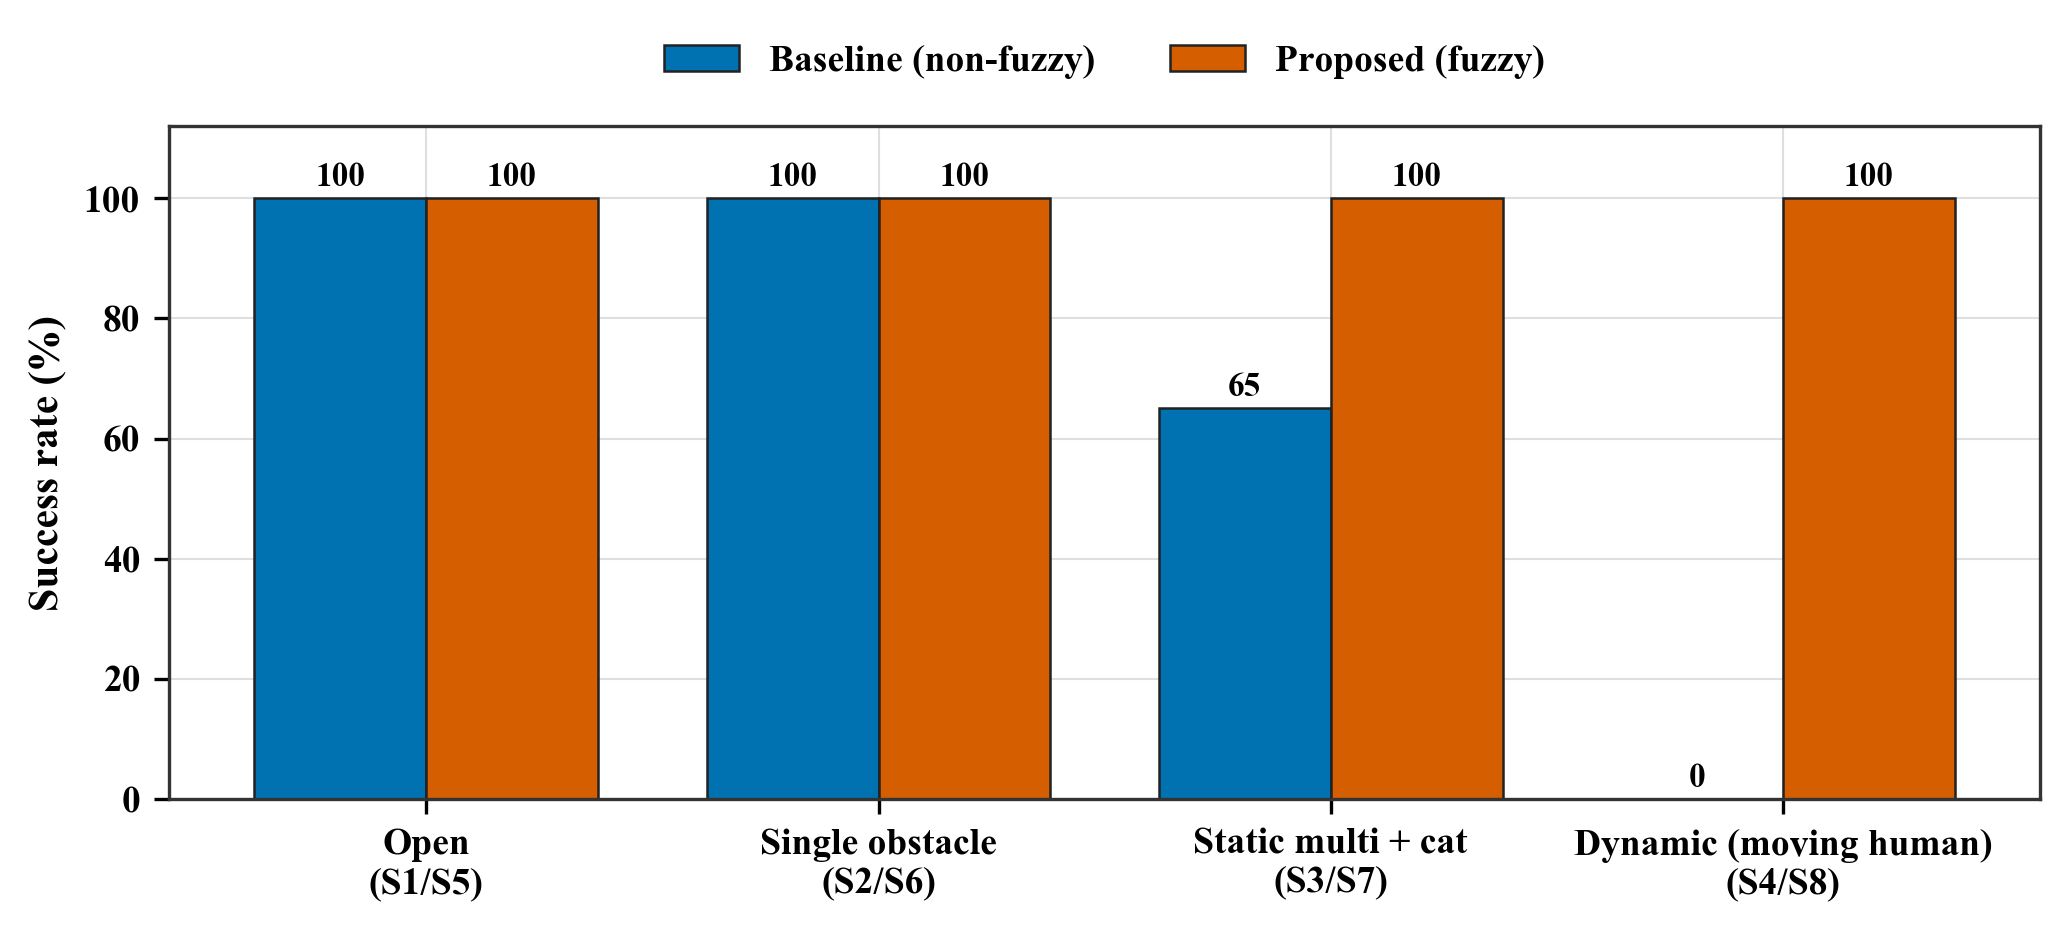
\includegraphics[width=0.85\textwidth]{gambar/4.3_fig_success_collision.png}
\caption{Tingkat keberhasilan (\textit{success rate}) pada keempat pasangan skenario, dikelompokkan berdasarkan konfigurasi \textit{baseline} (biru) dan \textit{proposed method} (oranye). S4 merupakan satu-satunya skenario yang tidak mencapai tingkat keberhasilan 100\%.}
\label{fig:keberhasilan_tabrakan}
\end{figure}

Tabel~\ref{tab:keberhasilan_tabrakan} dan Gambar~\ref{fig:keberhasilan_tabrakan} menunjukkan bahwa seluruh skenario, kecuali S4, mencapai tingkat keberhasilan dan tingkat bebas tabrakan sebesar 100\%. Seluruh skenario fuzzy (S5--S8) mempertahankan keberhasilan penuh tanpa satu pun kegagalan pada 40 \textit{trial} yang dilakukan. Dengan demikian, satu-satunya kegagalan yang tercatat dari total 80 \textit{trial} terjadi pada S4, yaitu skenario \textit{baseline} dengan keberadaan \textit{obstacle} dinamis, sehingga menghasilkan tingkat keberhasilan dan tingkat bebas tabrakan masing-masing sebesar 90\%.

Pemeriksaan lebih lanjut terhadap data mentah \texttt{results.csv} pada skenario S4 menunjukkan bahwa kegagalan tersebut terjadi pada \textit{trial} ke-9. Pada \textit{trial} ini, nilai \texttt{collision\_count} tercatat sebesar 1 dengan \texttt{hit\_obstacles} mengindikasikan \texttt{obstacle\_human\_1}, yaitu salah satu \textit{obstacle} manusia yang bergerak secara osilatif pada skenario tersebut. Sebaliknya, nilai \texttt{hit\_cat} tercatat sebesar 0, sehingga dapat dipastikan bahwa tabrakan tidak melibatkan kucing. Nilai \texttt{min\_clearance\_m} pada \textit{trial} ini sebesar $-0{,}227$~m, sesuai dengan definisi $c_\text{min}$ pada Persamaan~\ref{eq:min_clearance}, yang mengindikasikan adanya penetrasi fisik antara robot dan \textit{obstacle}.

Menariknya, parameter \texttt{goal\_reached} pada \textit{trial} yang sama tetap bernilai 1. Hal ini menunjukkan bahwa robot secara fisik berhasil mencapai titik tujuan, tetapi tetap dikategorikan gagal karena tidak memenuhi syarat \texttt{collision\_count=0} pada definisi \textit{success} sebagaimana dinyatakan pada Persamaan~\ref{eq:success}. Dengan kata lain, kegagalan tersebut bukan disebabkan oleh ketidakmampuan robot mencapai tujuan. Selain itu, nilai \texttt{stuck} yang tercatat sebesar 0 mengindikasikan bahwa kegagalan juga tidak disebabkan oleh kondisi robot yang macet maupun \textit{timeout}, melainkan semata-mata akibat peristiwa tabrakan yang terdeteksi berdasarkan data \textit{ground-truth} sepanjang lintasan.

Sebagaimana telah dijelaskan pada Subbab~\ref{sec:perangkat_keras} dan Subbab~\ref{sec:model_robot}, mekanisme deteksi tabrakan pada penelitian ini didasarkan pada perhitungan jarak \textit{ground-truth}, bukan pada kontak fisik antar-\textit{mesh}. Oleh karena itu, karena robot menggunakan model gerak kinematik \texttt{libgazebo\_ros\_planar\_move} yang tidak mensimulasikan dinamika kontak, robot secara visual masih dapat melanjutkan pergerakan menembus \textit{obstacle} meskipun peristiwa tersebut telah tercatat sebagai tabrakan dalam proses evaluasi.

Secara keseluruhan, hasil pada Tabel~\ref{tab:keberhasilan_tabrakan} menunjukkan bahwa \textit{pipeline} navigasi yang dikembangkan memiliki tingkat kestabilan yang tinggi, dengan tingkat keberhasilan mencapai 100\% pada tujuh dari delapan skenario pengujian. Lingkungan dengan \textit{obstacle} dinamis (S4/S8) tampak sebagai kondisi yang paling menantang dibandingkan skenario lainnya, mengingat satu-satunya kegagalan pada seluruh 80 \textit{trial} ditemukan pada pasangan skenario tersebut. Meskipun demikian, pada S8 yang merepresentasikan kondisi lingkungan yang setara dengan konfigurasi \textit{proposed method}, tingkat keberhasilan tetap terjaga pada nilai 100\%. Temuan ini menunjukkan bahwa penambahan mekanisme adaptasi fuzzy dan penanganan \textit{blind-spot} kucing tidak menurunkan performa keberhasilan navigasi secara keseluruhan.

Sebagaimana telah ditetapkan pada Subbab~\ref{sec:metode_statistik}, metrik \textit{success} dan \textit{collision-free} tidak dianalisis menggunakan uji Mann--Whitney U. Kedua metrik tersebut bersifat biner dan menunjukkan distribusi yang sangat terkonsentrasi pada nilai 1 di tujuh dari delapan skenario (\textit{ceiling effect}), sehingga tidak memiliki variabilitas yang memadai untuk menghasilkan pengujian statistik yang diskriminatif. Oleh sebab itu, analisis inferensial dalam penelitian ini difokuskan pada lima metrik kontinu, yaitu \texttt{min\_clearance\_m}, \texttt{time\_sec}, \texttt{avg\_linear\_vel}, \texttt{avg\_angular\_vel}, dan \texttt{path\_length\_m}, sebagaimana dibahas pada Subbab~4.4 hingga Subbab~4.8.

Setelah dipastikan bahwa sistem mampu mempertahankan tingkat keberhasilan navigasi pada hampir seluruh kondisi pengujian, pembahasan selanjutnya difokuskan pada aspek keselamatan melalui analisis margin \textit{clearance} minimum. Variabel ini merupakan ukuran utama dalam pengujian hipotesis penelitian dan akan dibahas secara lebih mendalam pada Subbab~4.4.
